\section{Iteration 3}
Wie bereits nach der ersten Iteration wurde dem Auftraggeber auch nach der zweiten Iteration
Anhand einer kurzen Demonstration der Entwicklungsstand präsentiert.

Folgende Punkte sind bei dabei rückgemeldet worden:
\begin{itemize}
    \item Die für Desktops optimiert Benutzerschnittelle entspricht den Vorstellungen und wirkt intuitiv.
    \item Da vom Auftraggeber keine echten \ac{THD} Werte zur Verfügung gestellt werden können,
          können diese weggelassen werden.
    \item Die Applikation soll um den in der Aufgabenstellung (Anhang \ref{anhang:aufgabenstellung}) beschrieben Use Case:
          ``Eine benutzerdefinierte Zeitspanne der Messwerte mittels vorgegebener
          Labels beschriften. Bsp.: («Backofen war von 09:31 – 10:15 aktiv»)`` soll implementiert werden.
    \item Die Übertragung der Messdaten mittels \ac{MQTT} soll,
          wie bereits in der Aufgabenstellung (Anhang \ref{anhang:aufgabenstellung}) verlangt, mit \ac{TLS} verschlüsselt werden.
\end{itemize}
In der letzten der drei Iterationen wurden diese finalen Anforderungen umgesetzt.
Die nächsten Abschnitte berichten darüber.

\subsection{Labeling}
Wie in Kapitel \ref{cap1} beschrieben, ist ein Ziel dieser Arbeit,
dass Messdaten für Supervised Learning aufbereitet werden können.
Dazu müssen diese mit Labels versehen werden.
Was grundsätzlich unter Labels zu verstehen ist, wird im Abschnitt \ref{state:supervised-learning} Supervised Learning erklärt.
Für diese Arbeit sollen Zeitabschnitte, während denen Messdaten erfasst wurden, mit Labels versehen werden.
Ein Label entspricht dabei einem Typ von Stromverbraucher wie beispielsweise einem Backofen oder einem Kühlschrank.

Die beiden dazugehöigen Anwenungsfälle sind in Abbildung \ref{fig:labeling} zu dargestellt.

\begin{figure}[H]
    \centering
    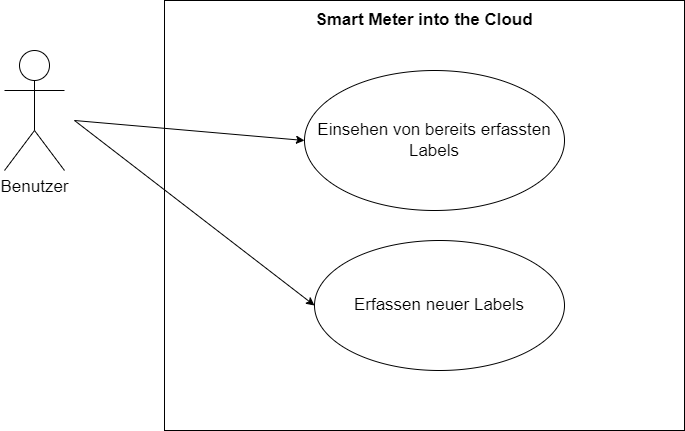
\includegraphics[width=1.0\textwidth]{gfx/labeling.drawio}
    \caption{Anwendungsfall Diagramm zu Labeling}
    \label{fig:labeling}
\end{figure}


\subsubsection{Benutzerschnittstelle}
% \subsection{Labeling}
% - Labeling:
% Labels graphisch darstellen
% Labels mittels UI hinzufügen

\subsubsection{API}
Was musste bei der api gemacht werden

\subsection{\ac{TLS} Verschlüsselung}

Mit \ac{TLS} können drei Sachen erreicht werden \parencite{what_is_tls}:

\begin{itemize}
    \item \texttt{Verschlüsselung}: Garantiert, dass gesendete Daten nicht von Dritten abgehört werden können.
    \item \texttt{Authentifizierung}: Versichert, dass die an der Kommunikation teilnehmenden Parteien, die sind für die sie sich ausgeben.
    \item \texttt{Integrität}: Verifiziert, dass gesendete Daten auf dem Sendeweg nicht durch Dritte geändert worden sind.
\end{itemize}

Erreicht wird dies, durch SSL Zertifikate \parencite{what_is_ssl_certificate}. Diese sind auf dem Server
installiert und werden durch eine \ac{CA} ausgestellt \parencite{what_is_ca}.
Dadurch wird die Authentifizierung eines Servers sichergestellt.
Diese \ac{CA} ist eine vertrauenswürdige Stelle\footnote{
    Beispielsweise Letsencrypt \parencite{letsencrypt_2021}
} welche sicherstellt, dass eine Domäne wirklich dieser Person gehört die das auch behauptet.
Um \ac{TLS} Verschlüsselung für die Entwicklung zu verwenden ist das jedoch nicht notwendig.
Dann kann mit sogenannten Self Signed Certificates gearbeitet werden \parencite{self_signed_cert}.
Der einzige Unterschied dabei ist, dass keine \ac{CA} das Zertifikat signiert, sondern, dass
dies selbst gemacht werden muss. In diesem Projekt wurde für die automatische Erstellung eines solchen
Zertifikates mkcert\footnote{https://github.com/FiloSottile/mkcert} verwendet.

Die Konfiguration des \ac{MQTT} Brokers kann einfach aus der Anleitung \parencite{mosquitto.conf_man_page_2021}
implementiert werden:

\begin{verbatim}
cafile /rootCA.pem
certfile /localhost+4.pem
keyfile /localhost+4-key.pem
\end{verbatim}

Den Clients\footnote{
    In diesem fall ist das der Fakemeter der die Daten verarbeitet und die verschiedenen
    Stromzähler welche die Daten senden.
} muss danach nur noch gesagt werden welcher \ac{CA} sie vertrauen können.
In diesem fall, ist dies ein Self Signed Certificate namens \texttt{rootCA.pem} das mittels
mkcert generiert wurde.

\subsection{Verifikation}

Um die korrekte Funktionalität der neu implementierten Anforderungen zu verifizieren, wurden
zwei neue End to End Tests implementiert. Diese verifizieren zum einen die Funktionalität der
Labelerstellung und zum anderen, ob die \ac{TLS} Verschlüsselung funktioniert (Abbildung \ref{fig:test-iteration-3}).

\begin{figure}[H]
    \centering
    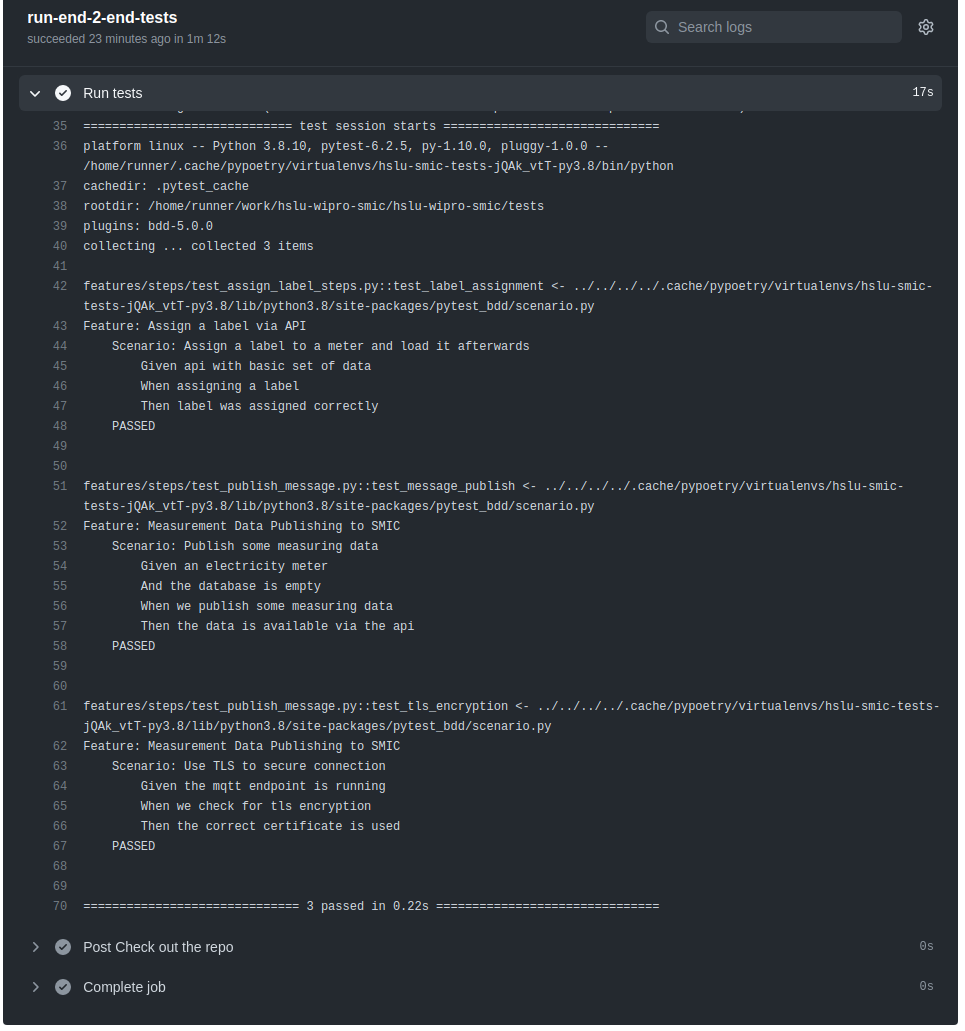
\includegraphics[width=1.0\textwidth]{gfx/testlog-iteration-2}
    \caption{
        Erweiterung der Tests um das Assignment der Labels und Testen der \ac{TLS} Verschlüsselung \parencite{randombenj_testlog_it_2_2021}.
    }
    \label{fig:test-iteration-3}
\end{figure}

\subsection{Schwierigkeiten}
Die Python Library `paho`, welche für die \ac{MQTT} Kommunikation verwendet wird, so zu konfigurieren,
dass sie die \ac{TLS} Verschlüsselung unterstützt, stellte sich als Schwierigkeit heraus.
Nach einiger Recherche, zeigte sich, dass `paho` ein unübliches \ac{TLS}
Verhalten aufweist \parencite{eclipse_paho_ssl_2019}.
Nachdem der Parameter \texttt{cert\_reqs=ssl.CERT\_NONE} gesetzt wurde, funktionierte
die \ac{TLS} Verschlüsselung dann auch.